\documentclass{amsart}
\usepackage[margin=12mm]{geometry}
\parindent = 0pt
\usepackage[svgnames]{xcolor}

\usepackage[skins,listings]{tcolorbox}

\NewTotalTCBox\keyword{ O{} v }{
  fontupper=\sffamily,
  nobeforeafter,
  skin=tile,
  tcbox raise base,
  top=0pt,bottom=0pt,left=0mm,right=0mm,
  colback=yellow!10!white,
  colupper=ForestGreen,
  #1}
{#2}

\lstdefinestyle{tikz}{style=tcblatex,
  classoffset=0,
  texcsstyle=*\color{blue},%
  deletetexcs={begin,end},
  moretexcs={,%
    pgfdeclarehorizontalshading,
    pgfuseshading,
    node,
    useasboundingbox,
    draw
  },%
  classoffset=1,
  keywordstyle=\color{MediumBlue},%
  morekeywords={tikzpicture,shade,fill,draw,path,node,child,line,width,rectangle},
  classoffset=2,
  keywordstyle=\color{ForestGreen},%
  morekeywords={solid,dot,list,affine,red,ghost, no}
}

\DeclareTCBListing{tikzcode}{ !O{} }{%
  skin=bicolor,
  colframe=NavyBlue,
  colbacklower=Lavender,
  colback=LightYellow,
  lefthand width=50mm,
  listing style=tikz,
  sidebyside,
  sidebyside gap=4mm,
  text and listing,
  text outside listing,
  tikz lower,
  #1
}

\usepackage{tikz}
\usetikzlibrary{decorations.markings,decorations.pathreplacing}

% \usepackage{calc}
% \input{pgfmanual-en-macros.tex}
% \RequirePackage{pgfmanual}

\tikzset{
  % default string colours
  affine colour/.initial=orange,
  affine color/.style={affine colour=#1},
  red colour/.initial=red,
  red color/.style={red colour=#1},
  ghost colour/.initial=gray,
  ghost color/.style={ghost colour=#1},
  ghost shift/.initial=1,
  solid colour/.initial=blue,
  solid color/.style={solid colour=#1},
  % KLRW node style
  klrw node/.style = {
     font=\scriptsize,
  },
  % string labels
  add string label/.style 2 args = {
    decoration = {
      markings,
      mark = at position 0 with {
        \node[below, text=\pgfkeysvalueof{/tikz/#1 colour}]{$#2$};
      },
    },
    preaction = { decorate }
  },
  add ghost label/.style = {
    decoration = {
      markings,
      mark = at position 1 with { \node[above, text=\pgfkeysvalueof{/tikz/ghost color}]{$#1$}; },
    },
    preaction = { decorate }
  },
  % red and affine red strings
  red/.style = {
    double=\pgfkeysvalueof{/tikz/red colour}!40,
    draw=\pgfkeysvalueof{/tikz/red colour},
    double distance=2pt,
    add string label={red}{#1}
  },
  affine/.style = {
    double=\pgfkeysvalueof{/tikz/affine colour}!40,
    draw=\pgfkeysvalueof{/tikz/affine colour},
    double distance=2pt,
    add string label={affine}{#1}
  },
  % solid strings
  solid/.style = {
     very thick,
     rounded corners,
     draw=\pgfkeysvalueof{/tikz/solid colour},
     preaction={
      draw ghost string,
      dashed,
      transform canvas={shift={(\pgfkeysvalueof{/tikz/ghost shift},0)}}
    },
    % add string label={solid}{#1},
    %add ghost label={#1},
  },
  solid/.default=,
  % ghost strings
  draw ghost string/.style ={
    draw=\pgfkeysvalueof{/tikz/ghost colour}
  },
  no ghost/.style={
    draw ghost string/.style = {
      draw = none,
      text = none
    }
  },
  double ghost/.style = {
    draw ghost string/.style = {
      draw=\pgfkeysvalueof{/tikz/ghost colour},
      double,
    }
  },
  % dots on strings
  dot/.style = {
    decoration={
      markings,
      mark=at position #1 with {
        \node[text=\pgfkeysvalueof{/tikz/solid colour}]{$\bullet$};
        \node[text=\pgfkeysvalueof{/tikz/ghost colour},
              xshift=\pgfkeysvalueof{/tikz/ghost shift}]{$\bullet$};
      },
    },
    postaction={
      decorate
    },
  },
  dot/.default=0.5,
}

\begin{document}

  The KLRW diagram package provides a series of TikZ style and \LaTeX\
  commands for drawing KLRW diagrams.

  \section{Strings in KLRW diagrams}

  Use the \keyword{solid} style to draw solid strings:

  \begin{tikzcode}
    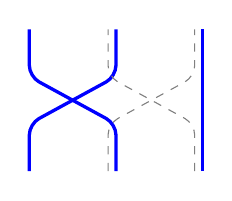
\begin{tikzpicture}
      \draw[solid](0,0)--++(0,0.6)--++(1.1,0.6)--++(0,0.6);
      \draw[solid](1.1,0)--++(0,0.6)--++(-1.1,0.6)--++(0,0.6);
      \draw[solid](2.2,0)--++(0,1.8);
    \end{tikzpicture}
  \end{tikzcode}

  By default, solid strings come with ghost strings. If a solid
  string does not have a ghost then add the style \keyword{no ghost}:

  \begin{tikzcode}
    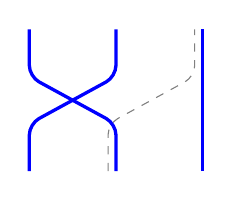
\begin{tikzpicture}
      \draw[solid](0,0)--++(0,0.6)--++(1.1,0.6)--++(0,0.6);
      \draw[solid, no ghost](1.1,0)--++(0,0.6)--++(-1.1,0.6)--++(0,0.6);
      \draw[solid](2.2,0)--++(0,1.8);
    \end{tikzpicture}
  \end{tikzcode}


  Optionally, you can specify the \keyword{residue} of a solid string,
  and its ghost, by giving it a value: \keyword{solid=i}. The labels for
  solid strings appear below the strings and the label for ghost strings
  appear above them.

  \begin{tikzcode}
    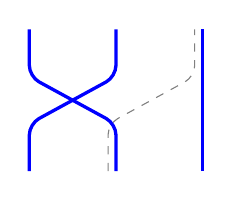
\begin{tikzpicture}
      \draw[solid=1](0,0)--++(0,0.6)--++(1.1,0.6)--++(0,0.6);
      \draw[solid=i, no ghost](1.1,0)--++(0,0.6)--++(-1.1,0.6)--++(0,0.6);
      \draw[solid](2.2,0)--++(0,1.8);
    \end{tikzpicture}
  \end{tikzcode}

  Dots can be added to a solid string, and its ghost, by using the
  \keyword{dot} style, \textit{which must appear before the other
  style commands}. By default, the dots appear in the middle of the
  string, which can be adjusted by giving \keyword{dot} a value between
  $0$ and $1$:

  \begin{tikzcode}
    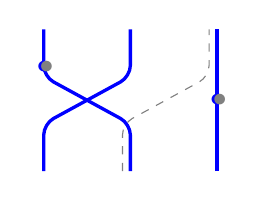
\begin{tikzpicture}
      \draw[solid=1](0,0)--++(0,0.6)--++(1.1,0.6)--++(0,0.6);
      \draw[solid=i, no ghost, dot=0.8](1.1,0)--++(0,0.6)--++(-1.1,0.6)--++(0,0.6);
      \draw[dot, solid](2.2,0)--++(0,1.8);
    \end{tikzpicture}
  \end{tikzcode}

  For multiple dots, use \keyword{dot/.list}$=\{...\}$:

  \begin{tikzcode}
    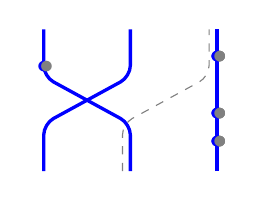
\begin{tikzpicture}
      \draw[solid=1](0,0)--++(0,0.6)--++(1.1,0.6)--++(0,0.6);
      \draw[solid=i, no ghost, dot=0.8](1.1,0)--++(0,0.6)--++(-1.1,0.6)--++(0,0.6);
      \draw[dot/.list={0.2,0.4,0.8}, solid](2.2,0)--++(0,1.8);
    \end{tikzpicture}
  \end{tikzcode}

  Finally, KLRW diagrams also contain \keyword{red} strings and
  \keyword{affine} red strings:

  \begin{tikzcode}
    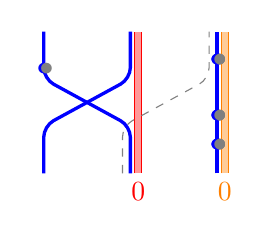
\begin{tikzpicture}
      \draw[red=0] (1.2,0)--+(0,1.8);
      \draw[affine=0] (2.3,0)--+(0,1.8);
      \draw[solid=1](0,0)--++(0,0.6)--++(1.1,0.6)--++(0,0.6);
      \draw[solid=i, no ghost, dot=0.8](1.1,0)--++(0,0.6)--++(-1.1,0.6)--++(0,0.6);
      \draw[dot/.list={0.2,0.4,0.8}, solid](2.2,0)--++(0,1.8);
    \end{tikzpicture}
  \end{tikzcode}

\end{document}

